% Prepared from the final Word manuscript, 7 November 2026.
% Official Springer Nature authoring class; pdfLaTeX; no line numbers.
\documentclass[pdflatex,sn-basic,Numbered]{sn-jnl}
\usepackage[T1]{fontenc}
\usepackage[utf8]{inputenc}
\usepackage{amsmath,amssymb,mathtools}
\usepackage{xcolor}
\usepackage{graphicx,longtable,booktabs,array,calc,multirow}
\usepackage{adjustbox}
\usepackage{microtype}
\usepackage{xurl}
\usepackage{fancyvrb}
\usepackage{caption}
\usepackage{placeins}
\usepackage{etoolbox}
\usepackage{bookmark}
\captionsetup{labelsep=space,labelfont=bf,font=small}
\captionsetup[figure]{name=Fig.}
\captionsetup[table]{name=Table}
\setcounter{secnumdepth}{3}
\setlength{\emergencystretch}{2em}
\urlstyle{same}
\hypersetup{hidelinks,pdftitle={Direct cognition problem: a semantic skeleton of mathematics and its growth},pdfauthor={Vasilii A. Gromov; Nikolai N. Evdokimov}}
\newcommand{\tightlist}{\setlength{\itemsep}{0pt}\setlength{\parskip}{0pt}}
\newcommand{\passthrough}[1]{#1}
\newsavebox{\displaybox}
\newcommand{\fitdisplay}[1]{\sbox{\displaybox}{$\displaystyle #1$}\ifdim\wd\displaybox>\linewidth\resizebox{\linewidth}{!}{\usebox{\displaybox}}\else\usebox{\displaybox}\fi}
\makeatletter
\newsavebox\pandoc@box
\newcommand*\pandocbounded[1]{\sbox\pandoc@box{#1}\ifdim\wd\pandoc@box>\linewidth\resizebox{\linewidth}{!}{\usebox\pandoc@box}\else\usebox\pandoc@box\fi}
\patchcmd\longtable{\par}{\if@noskipsec\mbox{}\fi\par}{}{}
\makeatother
\raggedbottom
\begin{document}
\title[A semantic skeleton of formal knowledge]{Direct cognition problem: a semantic skeleton of mathematics and its growth}
\subtitle{Epochs limit active premises while certificates preserve proofs}
\author[1]{\fnm{Vasilii A.} \sur{Gromov}}\email{stroller@rambler.ru}
\author*[1]{\fnm{Nikolai N.} \sur{Evdokimov}}\email{nevdokimov@hse.ru}
\affil[1]{\orgdiv{Laboratory for Semantic Analysis}, \orgname{National Research University Higher School of Economics}, \orgaddress{\street{11 Pokrovsky Bulvar}, \city{Moscow}, \postcode{109028}, \country{Russia}}}
\abstract{We study the direct cognition problem of formal knowledge: constructing a verifiable proof skeleton without a final target theorem under limited computational resources. We introduce a semantic skeleton of mathematics within a programme that distinguishes direct, inverse, and control cognition problems. Our continuous, generational generator separates a bounded active set, an archive of first proofs, and a library of closed fragments. The generator reversibly deactivates premises without deleting certificates. The selector measures how fragments shorten the expanded proof forest and accounts for definitions and overlaps; search need not activate stored fragments. An exponential lower bound on the number of explicitly expanded provable instances, together with a separate unboundedness result for the schema graph, limits exhaustive storage but does not imply that finite slices evade computation. A frozen panel of 144 source trajectories tests neutral continuation under resource guards. At its primary endpoint, learned half-selection with deferred replay increases mean novelty over ungated growth by 95.8\% and 30.3\% at propositional sizes 25 and 200, respectively, with eight positive pairs out of eight in each regime. A locked comparison across 16 sources and 963 human targets finds no confirmed adaptive advantage. The fixed extended repertoire initially covers 29 targets and averages 1.625 new common-residual targets at 90 operational processor-seconds. Network comparisons reveal modular structure and show how proof-edge conventions alter graph profiles. These results establish a certified method that preserves proofs and supports further growth, not a universal accelerator or an optimal skeleton.}
\keywords{formal knowledge, automated reasoning, semantic skeleton, proof hypergraph, theorem generation, Metamath}
\maketitle
\noindent\small ORCID (Nikolai N. Evdokimov): \url{https://orcid.org/0009-0003-3756-8281}\par\normalsize

\section*{1. Introduction}\label{introduction}
\addcontentsline{toc}{section}{1. Introduction}

Comparing the graph of all formally correct mathematical statements with the graph of those that humanity regards as theorems and lemmas \citep{MetamathSetMMPinned} reveals a striking difference (see Section 7.3). We call the latter object a semantic skeleton of mathematics. This article studies it and develops methods to generate it. This concept readily extends to any formalisable knowledge system, where we call it a semantic skeleton of formal knowledge. The skeleton provides a compact active representation through anchor statements and links to expandable proofs; it neither depicts the complete theorem space nor automatically discovers a system of mathematical concepts. Here, `semantic' means that the skeleton preserves formal statements, proof roles, and application conditions, whereas any substantive affinity with human mathematics requires a separate test. For knowledge-based reasoning, we ask which proved statements search should retain as premises under limited resources.

Our research programme distinguishes three cognition problems -- direct, inverse, and control cognition problems; this paper addresses the first. The \textbf{direct cognition problem} generates a proof skeleton without a final target theorem. We aim not merely to generate correct mathematical statements\footnote{Bachmair and Ganzinger \citep{BachmairGanzinger2001}, in \emph{Resolution Theorem Proving}, describe saturation through inference and redundancy criteria. Wernhard \citep{Wernhard2026}, in \emph{Generating Theorems by Generating Proof Structures}, studies target-free theorem generation. Section 2 distinguishes these foundations from the architecture and future-use test that we develop here.}, but to generate those that belong to the semantic skeleton. \textbf{The inverse problem} takes a particular statement and seeks intermediate lemmas that connect it to the existing base (current skeleton), to certify its status relative to the chosen formal system. This requires a proof of the statement, a proof of its negation, or a separate independence argument; unsuccessful search returns unknown. The \textbf{control problem} selects a growth regime to obtain a graph with desirable properties such as modularity, concentrated reuse, or a particular degree distribution. Tuning towards an external structural objective belongs to control, and success on a target theorem belongs to the inverse problem; neither supplies evidence that a topology emerges spontaneously.

The present paper addresses the direct problem by generating a semantic skeleton of mathematics under a fixed computational budget. In particular, it examines how activating library fragments affects continuous forward growth from axioms. We assess three independent outcomes: (1) how many new canonical formulae the generator discovers, (2) how much reuse costs, and (3) how many results match human statements. 

The paper proposes (1) a formal contract, (2) an executable architecture, and (3) a reproducible comparison. The contract distinguishes proof status, activity, and certificate preservation, as well as schemata and their explicit instances\footnote{A formal contract states checkable guarantees (Definition 1). Proof status records whether a certificate passes the checker; activity permits use as a premise. A certificate records replayable proof steps. A schema contains expression variables; an instance substitutes admissible expressions consistently. Preserving a certificate retains its proof steps and dependencies.}. The architecture supports continuous generational growth through a bounded active set, reversible deactivation, and an append-only certificate log; it separates the fragment library from decisions to activate fragment conclusions as premises. The comparison separates proof preservation, shorter expanded representations, and productive subsequent search. 

\section*{2. Related papers}\label{related-papers}
\addcontentsline{toc}{section}{2. Related papers}

The problem connects automated theory exploration, inference control, and proof reuse. Four distinctions guide comparisons: whether a method generates a statement together with its proof or first proposes a conjecture; whether it receives a final target; what it excludes from computation; and how it measures usefulness. These distinctions carry more weight than the mere presence of a graph, queue, or lemma library.

\subsection*{2.1 Saturation and search-resource limits}\label{saturation-and-search-resource-limits}
\addcontentsline{toc}{subsection}{2.1 Saturation and search-resource limits}

Bachmair and Ganzinger \citep{BachmairGanzinger2001}, in their handbook chapter \emph{Resolution Theorem Proving}, explain how saturation combines inference rules with redundancy criteria. Schulz \citep{Schulz2002}, in \emph{E --- A Brainiac Theorem Prover}, and Kov\'{a}cs and Voronkov \citep{KovacsVoronkov2013}, in \emph{First-Order Theorem Proving and Vampire}, describe how clause indices, scores, and simplification direct that search. Target-free forward inference therefore supplies background rather than our novelty claim. We retain a long-lived archive of checked consequences and assess the skeleton through new growth under bounded activity.

Riazanov and Voronkov \citep{RiazanovVoronkov2003LRS}, in \emph{Limited Resource Strategy in Resolution Theorem Proving}, adapt permissible clause weights to remaining time and search statistics. Their strategy directly precedes resource-based pruning. Logical redundancy and low expected computational return support different guarantees: a suitable redundancy criterion can preserve completeness, whereas a heuristic return estimate need not. Our age-based pruning protects earlier certificates but does not ensure fair future enumeration.

Hoder and Voronkov \citep{HoderVoronkov2011}, in \emph{Sine Qua Non for Large Theory Reasoning}, reduce the initial theory for a particular problem through SInE. Blanchette and colleagues \citep{BlanchetteEtAl2016}, in \emph{A Learning-Based Fact Selector for Isabelle/HOL}, learn fact relevance from earlier proof dependencies. Jakub\r{u}v and Urban \citep{JakubuvUrban2017}, in \emph{ENIGMA: Efficient Learning-Based Inference Guiding Machine}, rank clauses during search according to how they contribute to successful proofs. These studies distinguish how a prover initially chooses premises from how it controls search. We additionally distinguish storing a fragment from admitting its conclusion to a bounded active slot, without labelling success against a final target.

\subsection*{2.2 Theory exploration and the usefulness of new statements}\label{theory-exploration-and-the-usefulness-of-new-statements}
\addcontentsline{toc}{subsection}{2.2 Theory exploration and the usefulness of new statements}

Colton \citep{Colton2002}, in his monograph \emph{Automated Theory Formation in Pure Mathematics}, develops automated concept and conjecture discovery. Smallbone and colleagues \citep{SmallboneEtAl2017}, in \emph{Quick Specifications for the Busy Programmer}, present QuickSpec, which enumerates terms, tests conjectural equalities, and reduces redundancy through their dependencies. Claessen and colleagues \citep{ClaessenEtAl2013}, in \emph{Automating Inductive Proofs Using Theory Exploration}, combine such exploration with inductive proof in HipSpec. These systems show how auxiliary statements can support later work; our archive instead accepts each statement together with its checked derivation.

Johansson and colleagues \citep{JohanssonEtAl2014}, in \emph{Hipster: Integrating Theory Exploration in a Proof Assistant}, validate conjectures through Isabelle/HOL and assess interestingness against ordinary and stronger proof mechanisms. Singher and Itzhaky \citep{SingherItzhaky2021}, in \emph{Theory Exploration Powered by Deductive Synthesis}, combine symbolic enumeration, rewriting, congruence closure, and inductive checking in TheSy. Their bounded solver also examines mutual derivability. These studies motivate separate measures of novelty, proof status, and usefulness; our archive checks every accepted derivation, whereas our experiments assess continued growth rather than mutual derivability of complete theories.

McCasland, Bundy, and Smith \citep{McCaslandBundySmith2017}, in MATHsAiD: Automated mathematical theory exploration, describe theorem discovery from supplied axioms and definitions and distinguish it from proving a supplied goal. This distinction also frames our direct problem. We distinguish archived certificates, reusable fragments, and active premises in our experiments, and measure how much continued generation costs.

\subsection*{2.3 Generating proof structures: the closest predecessors}\label{generating-proof-structures-the-closest-predecessors}
\addcontentsline{toc}{subsection}{2.3 Generating proof structures: the closest predecessors}

Wernhard and Bibel \citep{WernhardBibel2024}, in \emph{Investigations into Proof Structures}, distinguish proof-tree size from minimal directed acyclic proof-graph size and study level-wise enumeration, theorem-size bounds, and bounded caches. Their analysis directly informs our generator. We extend the experimental focus to persistent certified growth and separately control archived proofs, reusable fragments, and active premises.

Wernhard \citep{Wernhard2026}, in \emph{Generating Theorems by Generating Proof Structures}, combines target-free enumeration, inductive levels, lemma synthesis through shorter proof representations, and comparison with human Metamath theorems. We build on this methodological precedent through continuous certified growth, reversible activity control, and prospective leases whose costs we measure. Our comparisons separate fragment recurrence from additional output when search admits fragment conclusions.

Rawson and colleagues \citep{RawsonEtAl2023}, in \emph{Lemmas: Generation, Selection, Application}, separate those three stages and compare structural usefulness scores with changes in proving work after lemma addition. Their tests motivate our distinction between shorter proof code and faster subsequent search. They assess lemmas through proof tasks; our principal trajectories instead continue without an external final target.

Wernhard and Zombori \citep{WernhardZombori2025}, in their preprint \emph{Mathematical Knowledge Bases as Grammar-Compressed Proof Terms: Exploring Metamath Proof Structures}, encode libraries through compressed proof terms, including parametrised fragments. Our code-length criterion scores particular closed first proofs, whereas a separate compiler derives general closed schemata from open modus-ponens programmes. The archive already shares subproofs. Consequently, shorter expanded forests measure the declared proof-term code rather than additional compression of the archive graph or universal human lemma value.

\subsection*{2.4 Acquired knowledge: from recurrence to computational return}\label{acquired-knowledge-from-recurrence-to-computational-return}
\addcontentsline{toc}{subsection}{2.4 Acquired knowledge: from recurrence to computational return}

Minton \citep{Minton1990Utility}, in \emph{Quantitative Results Concerning the Utility of Explanation-Based Learning}, measures how applicability checks and maintenance can outweigh gains from acquired knowledge. Our setting adds competition for a bounded number of active-premise slots. Frequent fragment occurrences establish reuse, but only a costed continuation test can assess whether access to those conclusions yields more new results. We therefore report code-length savings separately from computational return.

Kaliszyk and Urban \citep{KaliszykUrban2015}, in \emph{Learning-Assisted Theorem Proving with Millions of Lemmas}, select intermediate lemmas through acquisition cost, reuse, centrality, and greedy changes to the dependency graph. They also distinguish protocols by access to future proofs. Our selector recalculates overlaps using only the preceding forest, because earlier choices change the value of another fragment. After a run, we separately measure how many human statements the results cover; this diagnostic does not supply an independent holdout.

\subsection*{2.5 Trainable generators and growing libraries}\label{trainable-generators-and-growing-libraries}
\addcontentsline{toc}{subsection}{2.5 Trainable generators and growing libraries}

Wang and colleagues \citep{WangEtAl2023Lego}, in \emph{LEGO-Prover: Neural Theorem Proving with Growing Libraries}, build and reuse verified auxiliary skills while solving formal tasks. Yang and colleagues \citep{YangEtAl2023}, in \emph{LeanDojo: Theorem Proving with Retrieval-Augmented Language Models}, combine premise retrieval with search and track fact availability. These systems inform future uses of a skeleton for target-driven reasoning. Our historical direct-growth panels start from axioms, whereas the native extensions inherit a certified source library. Neither calls a language model for formulae or fragments.

Poesia and colleagues \citep{PoesiaEtAl2024}, in \emph{Learning Formal Mathematics from Intrinsic Motivation}, jointly learn conjecturing and proving in MINIMO from an initial axiomatisation. Ota and colleagues \citep{OtaEtAl2026}, in their preprint \emph{Self-Supervised Theorem Discovery in a Formal Axiomatic System}, turn discovered theorems into prover actions and select them through generalisation and difficulty of rediscovery. Both systems create their own search targets. Our generator instead continues forward without a trainable target-setting loop.

Lin and colleagues \citep{LinEtAl2024}, in \emph{ATG: Benchmarking Automated Theorem Generation for Generative Language Models}, assess generated theorems partly through their usefulness for subsequent proving. We test neutral direct continuation and exact matches to human statements. This choice measures further target-free growth; independent goal-directed tasks would test the complementary inverse problem.

\subsection*{2.6 Prover cooperation and graphs of mathematical libraries}\label{prover-cooperation-and-graphs-of-mathematical-libraries}
\addcontentsline{toc}{subsection}{2.6 Prover cooperation and graphs of mathematical libraries}

Tomaszuk and colleagues \citep{TomaszukEtAl2023}, in \emph{MMLKG: Knowledge Graph for Mathematical Definitions, Statements and Proofs}, represent the existing Mizar library as a knowledge graph. Li and colleagues \citep{LiEtAl2026}, in their preprint \emph{The Network Structure of Mathlib}, distinguish dependency levels and relate observed centrality to formalisation infrastructure. These studies motivate a graph-level account of mathematical libraries. Our generator additionally requires joint premises and expandable certificates; high degree, short paths, or a compact projection cannot replace those proof conditions.

\subsection*{2.7 Position of this work}\label{position-of-this-work}
\addcontentsline{toc}{subsection}{2.7 Position of this work}

Our method assigns each proven formula three distinct roles: an archived result, a reusable library entry, and a possible active premise. Certificate replay checks the first role, past savings in proof code help select reusable entries, and neutral continuation measures future use. Structural synthesis adds another route to library entries through checked deduction. The contribution combines these mechanisms with explicit access permissions and tests their incremental effects over fixed controls.

\section*{3 Formal model and outcome criteria}\label{formal-model-and-outcome-criteria}
\addcontentsline{toc}{section}{3 Formal model and outcome criteria}

\subsection*{3.1 Calculus and proof state}\label{calculus-and-proof-state}
\addcontentsline{toc}{subsection}{3.1 Calculus and proof state}

A proof certificate records elementary inferences and substitutions that a checker can replay from the initial base. We call a statement proven once its certificate passes those checks, and active when the generator may use it as a premise. A schema contains variables that stand for admissible expressions; an instance replaces those variables consistently. A configuration fixes the language, proof rules, and contextual requirements:

\[\fitdisplay{\mathcal{C} = (\Sigma,\Gamma,\Re,\nu,\Xi),}\]

where \(\Sigma\) specifies the language, \(\Gamma\) denotes the initial axioms or schemata, \(\Re\) contains the rules, \(\nu\) maps each statement to its declared canonical form, and \(\Xi\) describes contextual restrictions. In systems with quantifiers and hypotheses, each vertex includes the necessary context, variable types, and admissible-substitution conditions alongside its formula. Formula identity alone therefore need not identify the full proof state.

A typed hypergraph\footnote{A typed directed hypergraph records statements as vertices, together with their variable types, hypotheses, and side conditions. A directed hyperedge joins an ordered group of premises to one conclusion and records the rule and substitution. Its premise order identifies rule roles; the inference requires those premises jointly.

  For modus ponens (MP), the minor premise \(p\) and major premise \(p \rightarrow q\) jointly yield \(q\); neither premise alone supplies that inference.} \(H = (V,E)\) provides the primary representation. We record a rule application as

\[\fitdisplay{e = (p_{1},\ldots,p_{k};\rho;\sigma;\chi;q),}\]

where \(p_{i}\) denotes premises in role order, \(\rho\) denotes the rule, \(\sigma\) denotes the substitution, \(\chi\) contains side conditions, and \(q\) denotes the conclusion. Each hyperedge requires all its premises jointly, whereas alternative hyperedges represent different derivations of the same conclusion. The representation thus preserves the distinction between jointly necessary premises and alternative proofs.

To canonicalise means to remove only the declared redundancy of notation. In the implicational fragment, the procedure normalises variable names by first occurrence without identifying arbitrary logically equivalent formulae. A canonical identifier therefore does not turn a vertex into a semantic equivalence class.

\subsection*{3.2 Skeleton contract}\label{skeleton-contract}
\addcontentsline{toc}{subsection}{3.2 Skeleton contract}

\textbf{Definition 1.} A certified proof skeleton consists of a triple

\[\fitdisplay{\mathcal{S} = (S,\Omega,\mathsf{E}\mathsf{x}\mathsf{p}\mathsf{a}\mathsf{n}\mathsf{d}),}\]

with the following properties. A finite certificate in \(\Omega\) supports every anchor vertex \(v \in S\); certificate dependencies satisfy well-foundedness; \(\mathsf{E}\mathsf{x}\mathsf{p}\mathsf{a}\mathsf{n}\mathsf{d}\) expands an anchor-lemma reference into a proof from the permitted initial base; and every elementary step passes rule and side-condition checks. Together, these requirements let a checker recover each anchor independently from that base.

The contract does not require every known alternative proof. An implementation may preserve one correct witness, several variants with different costs, or a common structure that shares subproofs. Deleting the sole expandable witness nevertheless violates the contract unless another certified reconstruction remains available.

`Semantic' carries a restricted operational meaning here. The skeleton preserves formal statements, their proof roles, and application conditions, whereas we must test separately whether the skeleton resembles how humans organise mathematics. In particular, provable equivalence among all theorems relative to a common theory provides too coarse a relation for identifying useful anchor lemmas.

\subsection*{3.3 Reconstruction and new growth}\label{reconstruction-and-new-growth}
\addcontentsline{toc}{subsection}{3.3 Reconstruction and new growth}

Proof expansion and new growth serve distinct purposes:

\[\fitdisplay{\mathsf{E}\mathsf{x}\mathsf{p}\mathsf{a}\mathsf{n}\mathsf{d}(\mathcal{S},v) \rightarrow \pi_{v},\quad\quad\mathsf{G}\mathsf{r}\mathsf{o}\mathsf{w}(\mathcal{S},b) \rightarrow \Omega_{b}.}\]

The first operator returns a certificate for an existing anchor. The second performs forward inference under budget \(b\) without a final target formula, using the initial axioms, selected anchors, and its own new consequences. Vertices that serve only as proof support do not automatically enter the available premise set, so archival presence alone does not confer search activity.

New-growth counts exclude rediscovery of formulae that the archive already contains. Let \(\Omega_{0}\) denote the common initial archive from which the comparison policies choose anchors, and define the main direct-continuation measure as

\[\fitdisplay{N_{b}(\mathcal{S} \mid \Omega_{0}) = \left| V(\Omega_{b})\setminus V(\Omega_{0}) \right|.}\]

This measure counts syntactic novelty under the declared canonicalisation, even after earlier formulae leave the active skeleton. It does not establish mathematical significance for every new result.

An external set \(T\) supplies a supplementary measure of new exact matches:

\[\fitdisplay{M_{b}(\mathcal{S},T \mid \Omega_{0}) = \left| T \cap (V(\Omega_{b})\setminus V(\Omega_{0})) \right|.}\]

The later native tests use typed one-way coverage with mandatory distinct-variable conditions. For source block \(j\), let \(T\) denote the external reference and let \(C_{T}(S_{j,m},0)\) denote the statements that method \(m\) covers before further search. We freeze a common residual

\[\fitdisplay{R_{j} = T\setminus \bigcup_{m}C_{T}(S_{j,m},0),\quad\quad Q_{j}(m,h) = \left| R_{j} \cap C_{T}(S_{j,m},h) \right|.}\]

The observer measures coverage of committed results; it supplies no premise, reward, or proposed conclusion. The residual removes every method's initial coverage advantage within a block. Counts of \(Q_{j}\) test new reference capability, whereas \(N_{b}\) counts syntactically new formulae outside the common archive. Neither measure substitutes for the other, and exact matches remain a separate readout.

Resource accounting distinguishes the active set and reserve from the library, proof support, and archive. We measure their sizes separately, together with peak memory for the entire process; a fixed premise count does not imply fixed total memory. The principal size bounds \(L = 25,200\) count every syntax-tree vertex, not only leaves, and therefore constrain a different quantity from the active-set limit.

\subsection*{3.4 Useful skeletons and empirical Pareto sets}\label{useful-skeletons-and-empirical-pareto-sets}
\addcontentsline{toc}{subsection}{3.4 Useful skeletons and empirical Pareto sets}

A useful skeleton preserves checked proofs and supports further inference within the declared budget. The proof requirements guarantee the first property; neutral continuation tests the second. This operational criterion links proof preservation to the work that the retained library supports.

For each policy and anchor cap, we record a triple: the measured cost of constructing and using a skeleton, the bytes in its proof-backed package, and the new schemata that it generates during continuation. One setting dominates another only when it uses no more CPU or package bytes, yields at least as many new schemata, and improves at least one coordinate. The empirical Pareto set contains the nondominated settings within the declared finite comparison grid. This definition avoids assigning an arbitrary exchange rate between a byte, a CPU-second, and a new formula.

We compare settings only within one logic--size regime, one source ceiling, one continuation horizon, and a common exclusion archive. Package bytes include both anchors and certificate support; an anchor count alone omits that support. 

\section*{4 Limits of exhaustive explicit construction}\label{limits-of-exhaustive-explicit-construction}
\addcontentsline{toc}{section}{4 Limits of exhaustive explicit construction}

The combinatorial argument depends on the unit of storage. Let \(T_{L}\) contain the syntactically distinct formulae over one fixed letter \(p\) that admit proofs in which every formula, including axiom instances, contains at most \(L\) syntax-tree vertices. Size counts syntax-tree vertices, and the calculus contains the schemata \(K:A \rightarrow (B \rightarrow A)\) and \(S:\lbrack A \rightarrow (B \rightarrow C)\rbrack \rightarrow \lbrack(A \rightarrow B) \rightarrow (A \rightarrow C)\rbrack\), together with modus ponens. The resulting bound concerns explicit formula instances under these conventions.

\textbf{Theorem 1.} For every integer \(m \geq 0\),

\[\fitdisplay{|T_{18m + 17}| \geq {Cat}_{m},\quad\quad{Cat}_{m} = \frac{1}{m + 1}\binom{2m}{m} \sim \frac{4^{m}}{\sqrt{\pi}\, m^{3/2}}.}\]

These conclusions contain \(4m + 3\) syntax-tree vertices and admit proofs with at most two applications of modus ponens along any path from an axiom instance. Appendix A presents the full proof and intermediate size calculations, using standard Catalan enumeration \citep{FlajoletSedgewick2009}.

Exhaustive representation with a separate record for each such formula requires exponentially many records in \(L\). No fixed total capacity can accommodate that representation for every increasing \(L\). This output-volume bound does not supply a new lower bound on the complexity of finding a single proof, and it permits streaming output, growing storage, and exhaustive computation of any fixed finite slice.

The generator needs a separate schema-level bound. Every \(F \rightarrow F\) instantiates the single schema \(A \rightarrow A\), so the explicit family behind Theorem 1 collapses under schema storage. Its exponential bound therefore \textbf{does not transfer} to the number of canonical schemata in the archive.

\textbf{Theorem 2.} Let \(H_{d}^{sch}\) contain \(K\) and every most general result of schematic modus ponens up to depth \(d\), with separate renaming of premise variables and canonicalisation only up to renaming. With no size or width limits, subsumption, or pruning,

\[\fitdisplay{|V(H_{d}^{sch})| \geq d + 1.}\]

Appendix A proves the claim. Together, the bounds establish why an ever-growing exact graph eventually exceeds fixed retained capacity, distinguishing explicit instances from canonical schemata. They motivate a design that limits active work and preserves proof certificates separately. Appendix A details the assumptions, pair counts, and finite restrictions.

\section*{5 Continuous skeleton and proof library}\label{continuous-skeleton-and-proof-library}
\addcontentsline{toc}{section}{5 Continuous skeleton and proof library}

\subsection*{5.1 Continuous growth with distinct states}\label{continuous-growth-with-distinct-states}
\addcontentsline{toc}{subsection}{5.1 Continuous growth with distinct states}

The continuous variant keeps one generator across epochs and reserves no compulsory time share for a second branch. We track its state as

\[\fitdisplay{X_{e} = (A_{e},P_{e},D_{e},\Omega_{e},\mathcal{I}_{e},B_{e}),}\]

where \(A_{e}\) contains active premises, \(P_{e}\) holds the passive queue of proven candidates, \(\Omega_{e}\) contains the certificate archive, \(\mathcal{I}_{e}\) contains working indices, \(B_{e}\) denotes remaining resources, and \(D_{e}\) contains root identifiers for closed library fragments whose certificates reside in \(\Omega_{e}\). The program defines retained anchors as \(S_{e} = A_{e} \cup D_{e}\), without an additional independent state component. The two sets serve distinct purposes: \(A_{e}\) supplies search premises, whereas \(D_{e}\) stores references to multistep proofs that the checker verified. Their ancestor proof support \(Anc(A_{e} \cup D_{e})\) serves checking and expansion, not an additional active base.

The archive grows through new canonical statements and their first proofs. Only the initial axioms receive permanent protection in the working set. The policy retains other active formulae for finite periods and extends those periods when a formula contributes to the first proof of a new result; library-selected formulae receive a separate finite period. Deactivation removes a formula from search indices but preserves its archive entry. If search rediscovers that formula, the policy can return it to the passive queue after a specified delay and within a return quota, measuring its new age from queue re-entry rather than old proof depth. These operations neither change the certificate nor turn a derived lemma into an axiom.

Explicit limits constrain active derived formulae and passive candidates after every layer. The policy first preserves the new search frontier, then accounts for finite library-retention periods and recent productive use. Per-layer selection width and total active-set size remain separate parameters. Since the archive retains every entry, bounded activity does not imply constant total memory.

\subsection*{5.2 Utility of a reusable proof fragment}\label{utility-of-a-reusable-proof-fragment}
\addcontentsline{toc}{subsection}{5.2 Utility of a reusable proof fragment}

A closed fragment represents a particular first proof of a lemma with initial axioms at its leaves. Closure excludes unproven open premises, not schema variables; expansion follows each internal vertex's archived premises in their original order. This coding stage names existing proofs. The separate structural compiler below generalises short open proof programmes and derives their closed implication schemata. Both routes retain elementary certificates and leave the original consequence relation unchanged.

Fragment cost accounts for repeated premise positions. Let \(R_{e}\) denote a finite set of recent proofs for selection, and let \(pa(v)\) denote the ordered parent list of vertex \(v\), allowing repeated entries. Counting each premise occurrence with its multiplicity gives the expanded proof-term size

\[\fitdisplay{t(v) = 1 + \sum_{p \in pa(v)}^{}t(p).}\]

The unit counts an axiom name, a rule application, or a fragment reference. For a chosen library \(D\), define

\[\fitdisplay{c_{D}(v) = \left\{ \begin{matrix}
1, & v \in D, \\
1 + \sum_{p \in pa(v)}^{}c_{D}(p), & v \notin D,
\end{matrix} \right.\ }\]

\[\fitdisplay{d_{D}(v) = 2 + \sum_{p \in pa(v)}^{}c_{D}(p).}\]

The quantity \(d_{D}(v)\) includes a definition header and its root instruction, whereas references to other definitions must follow the original well-founded dependencies. Thus the encoding gain for the proof forest accounts for both references and definitions:

\[\fitdisplay{G(D;R_{e}) = \sum_{v \in R_{e}}^{}t(v) - \left\lbrack \sum_{v \in R_{e}}^{}c_{D}(v) + \sum_{v \in D}^{}d_{D}(v) \right\rbrack.}\]

The selector admits fragments only while they reduce code length; it need not fill its quota. Candidates comprise multistep proofs of height at least two that occur at least twice in the expanded forest; a bounded pool ranks them by how much each could reduce repetition. The greedy selector then adds the fragment with the largest positive increment in \(G\) and recalculates overlaps. The selector stops when no positive increment remains, so the procedure searches only a bounded candidate pool and does not guarantee optimal compression.

\textbf{Lemma 1 (library expansion).} For a finite acyclic archive, this encoding expands into the original forest of first proofs. If selection starts from an empty library and admits only strictly positive increments in \(G\), its final gain on the training forest remains non-negative. Appendix B.5 proves the lemma.

The lemma certifies exact recovery of the original proofs and a non-negative code-length gain on the selection forest. The gain \(G\) measures savings in expanded proof-term symbols; the archive already shares identical subproofs. The continuation experiments separately measure whether library conclusions improve future search under a CPU budget.

\subsection*{5.3 Continuous construction cycle}\label{continuous-construction-cycle}
\addcontentsline{toc}{subsection}{5.3 Continuous construction cycle}

A generation denotes a layer of new consequences, whereas an epoch denotes a point at which the program updates search state. Epoch number does not equal minimum proof height from the initial axioms. Unlike earlier restarts from selected anchors, this algorithm preserves one generator and its unfinished work; the experimental protocol specifies the retention periods, quotas, and bounds that govern that continuity.

\textbf{Algorithm 1. Continuous certified growth.}

\begin{enumerate}
\def\labelenumi{\arabic{enumi}.}
\tightlist
\item
  Check the initial axioms or inherited certified library, create the working indices, and initialise the archive and reusable dictionary.
\item
  While resources permit another layer, select an admissible frontier from the queue according to the fixed policy and its tie-breaking rule.
\item
  Process available rule applications. Check substitutions and side conditions, and canonicalise conclusions. Store a first proof for each new formula; handle rediscovery separately without increasing the new-formula count.
\item
  Update productive-use records and finite retention periods. Apply active-set and queue bounds while preserving certificates for inactive formulae. Return eligible rediscoveries to the queue subject to the specified delay and quota.
\item
  At the designated epochs, select a library from the preceding proof forest. In the active variant, apply bounded retention to its conclusions; in the passive variant, leave search state unchanged.
\item
  Store the new certificate increment and state snapshot. Credit only a fully completed layer within budget, and record the stopping reason.
\end{enumerate}

At a library-review point, the structural extension may add checked lemma schemata before the upper codec runs. It preserves the preceding interface and charges new definitions; it does not replace the accumulated generator with a new search from a hand-picked theorem list. 

Epochs limit active premises while certificates preserve proofs.

The algorithmic budget includes fragment selection, index updates, internal checking, and storage. The independent checker replays the complete log after the experiment; we account for its cost separately. The pseudocode consequently specifies dependency order among operations, not equal execution times for successive layers.

\subsection*{5.4 Soundness and the limit of the guarantee}\label{soundness-and-the-limit-of-the-guarantee}
\addcontentsline{toc}{subsection}{5.4 Soundness and the limit of the guarantee}

Every archive certificate expands to the initial base provided the axioms satisfy the configuration, each new step passes checking, and each reference points to an earlier certified vertex. Appendices B.1--B.2 state the formal guarantees and prove them. These guarantees preserve existing proofs when the policy deactivates premises, but do not ensure complete enumeration: an inactive premise can prevent a useful future rule application.

Adding a provable lemma does not strengthen the underlying logic, but can change which proofs the available resources can reach \citep{CookReckhow1979}. Under size and height bounds, we must account explicitly for intermediate formulae when we expand proofs; Appendix B and Section G.1 provide the full resource conditions and a specific identity example. Complete finite saturation additionally requires fair processing of every rule application that becomes available, a guarantee that the present bounded policy does not establish.

\subsection*{5.5 Learned pair selection with deferred replay}\label{learned-pair-selection-with-deferred-replay}
\addcontentsline{toc}{subsection}{5.5 Learned pair selection with deferred replay}

The later variant controls pairs of candidate premises before it unifies them. A frozen model scores only premise syntax and existing first-proof heights; it never inspects a proposed conclusion. Its training labels mark first-proof ancestry that supports an earlier compression dictionary. The policy retains roughly half of compatible candidates, includes a fixed exploratory share, and preserves their production traversal order. Thus it predicts a corridor towards useful proof support rather than the truth of an unseen theorem.

Deferred replay retains some skipped pairs in a bounded queue. Each epoch can test up to 128 ready pairs and reserve up to four ordinary premise slots to restore missing parents. A replay uses only currently active, certified premises; it does not introduce a new axiom or activate cold proof support. Queue capacity, overflow, and the cost of scores remain explicit. This mechanism delays the point at which the hard filter saturates while preserving the same elementary proof checker.

The policy constructs an archive, then extracts proof-backed anchor packages for neutral continuation. Source work, package choice, and continuation enter the reported chain CPU cost. Training and the later independent audit enter separate accounts. Code-length gain chooses candidate support, and continued growth measures operational usefulness. These separate tests allow a compact package to succeed without claiming that every retained formula belongs to a unique mathematical core.

\subsection*{5.6 Additional compression above the accumulated library}\label{additional-compression-above-the-accumulated-library}
\addcontentsline{toc}{subsection}{5.6 Additional compression above the accumulated library}

The upper codec preserves a base dictionary \(D_{0}\) and adds a definition only when its joint marginal gain remains positive. It recalculates nested references and definition costs after each addition and imposes no target dictionary size. For an eligible fragment, let \(r\) count its expanded occurrences in the current forest and dictionary bodies, and let \(b\) count the symbols in its current body. The exact saving under this code equals

\[\fitdisplay{\Delta(v \mid D) = (r - 1)(b - 1) - 2.}\]

The two charged symbols account for a new definition's root and header after the reference savings. Appendix K.1 proves this identity and its telescoping guarantee. Positive increments improve the previous encoding, even when \(D_{0}\) already contains mandatory entries; they do not guarantee a globally shortest code, fewer archive bytes, or faster future inference.

\subsection*{5.7 Structural synthesis of general lemma schemata}\label{structural-synthesis-of-general-lemma-schemata}
\addcontentsline{toc}{subsection}{5.7 Structural synthesis of general lemma schemata}

The structural layer abstracts a short MP proof tree, replaces its boundary by hypotheses, and considers possible equalities among those hypotheses. Joint typed unification solves all MP constraints together. For each consistent programme and order of its distinct boundary hypotheses, the compiler applies the deduction theorem and derives a closed implication schema. The generalisation rule (Gen) cuts an open fragment: the compiler never moves a deduction step through unrestricted Gen.

For example, a programme with boundary \(p\), \(p \rightarrow q\), and \(q \rightarrow r\) concludes \(r\). An appropriate discharge order yields

\[\fitdisplay{(p \rightarrow q) \rightarrow \left( (q \rightarrow r) \rightarrow (p \rightarrow r) \right).}\]

The compiler recovers this familiar composition law without a human theorem target. It expands every new step through ax-1, ax-2, and ax-mp, or invokes an existing checked schema through an explicit admissible instance. All output certificates pass the native checker and the independent Metamath verifier. Proposition K.2 states the proof obligation; this compiler implements the standard deduction construction rather than a new deduction theorem.

The catalogue distinguishes a requested principal formula from the actual schema that its certificate supplies. A more general stored schema may cover several requests, so we deduplicate delivered statements and their applicability frames. This distinction explains why candidate counts and delivered-rule counts need not coincide. The finite grammar and size guards bound the actual construction, not all possible useful lemmas.

\subsection*{5.8 Fixed structural repertoire}\label{fixed-structural-repertoire}
\addcontentsline{toc}{subsection}{5.8 Fixed structural repertoire}

The final native architecture combines the cumulative constructor and positive-marginal codec with a finite structural repertoire. A common grammar delivers 217 checked schemata through three open MP nodes, including 16 short outputs through two nodes. The fixed quota-matched variant adds 12 extended outputs that the fixed ranking selects using pooled earlier development profiles. It uses no held-out theorem to select those rules. This fixed repertoire supplies a reproducible working configuration, not an optimum over all possible libraries.

The locked comparison separately tests whether the source history should change those 12 outputs, versus fixed, random, and whole-catalogue alternatives. The adaptive score belongs to that comparative experiment rather than the recommended architecture. Appendix K.6 specifies it fully, and the results retain its registered outcome.

\subsection*{5.9 Search permissions after the library freezes}\label{search-permissions-after-the-library-freezes}
\addcontentsline{toc}{subsection}{5.9 Search permissions after the library freezes}

The neutral test receives only declared interface statements as premises. It cannot use certificate-only support for sampling, subsumption, or rejecting a rediscovery as already known. If search derives a hidden support statement again, the checker first validates a new witness from currently permitted parents; only then does the statement gain search rights. A separate log retains that witness even when the old archive already stores the same statement.

The neutral continuers reset learned scores, deferred queues, and reuse counters. They apply either uniform premise sampling or the same fixed mixture of uniform, bridging, contracting, and frontier sampling to every arm. They retain admitted future results without the constructor's rot-pruning or active cap. Thus this test assesses a library's use under a common engine, not the effect of running each builder's controller longer. The mixed engine retains an identifier-dependent frontier preference, so the experiment concerns delivered representations rather than an invariant semantic functional.

\section*{6 Materials and methods}\label{materials-and-methods}
\addcontentsline{toc}{section}{6 Materials and methods}

\subsection*{6.1 Formal systems and the scope of the tests}\label{formal-systems-and-the-scope-of-the-tests}
\addcontentsline{toc}{subsection}{6.1 Formal systems and the scope of the tests}

The historical propositional panels use \(\rightarrow ,\neg\) with three axiom schemata:

\[\fitdisplay{\begin{matrix}
{ax}_{1}:A \rightarrow (B \rightarrow A), \\
{ax}_{2}:\lbrack A \rightarrow (B \rightarrow C)\rbrack \rightarrow \lbrack(A \rightarrow B) \rightarrow (A \rightarrow C)\rbrack, \\
{ax}_{3}:(\neg A \rightarrow \neg B) \rightarrow (B \rightarrow A),
\end{matrix}}\]

Schematic modus ponens renames premise variables apart before it unifies them. The modal condition adds the normal K axiom \(\square(A \rightarrow B) \rightarrow (\square A \rightarrow \square B)\) and necessitation for theorems. These two configurations differ in language, axioms, and rules together, so their contrast does not isolate a causal effect of logic alone.

The size bound \(L \in \{ 25,200\}\) counts abstract-syntax-tree nodes in each canonical formula that the generator stores. 

An independent checker traces each new result to the original axioms. It implements its own canonical forms, occurs-check unification, and rule checks without importing the generator's corresponding code. The audit validates one first proof per vertex, not the complete set of alternative proofs.

Each random initial scheduler state defines one trajectory and hence one repeat. In the continuation experiments, a common source archive defines a block within which we pair the ways of choosing anchors. Thousands of formulae along one trajectory do not supply thousands of independent observations.

\subsection*{6.2 Native development and the one-shot holdout}\label{native-development-and-the-one-shot-holdout}
\addcontentsline{toc}{subsection}{6.2 Native development and the one-shot holdout}

The native tests inherit a certified 2,708-statement library on the explicit basis that the network study specifies. They continue the cumulative constructor rather than rebuild that source from axioms. The constructor retains its learned half-filter on supported implication/negation terms, intrinsic fallback scores on other native syntax, deferred opportunities, four ordinary fragment slots, and a cap of 128 active derived premises. Rot-pruning deactivates an unleased, never-used premise after eight idle blocks; cap enforcement can deactivate other premises as well. Neither operation deletes its certificate.

A development comparison uses six new states of the random number generator (RNG) for source construction, two neutral continuers, and nested horizons of one, three, and eight growth CPU-seconds. Its reference contains 919 unique compatible closed native statements, 34 of which axiom instances already cover. That reference previously informed development and cannot supply an independent holdout. We retain it to diagnose the mechanism and motivate the frozen test, not to confirm the adaptive claim.

For the one-shot test, Wernhard's POI supplies an external benchmark of 1,374 implication-form propositional theorems from Metamath \citep{Wernhard2026}. We exclude 402 alpha-exact matches to the preceding reference after unfolding the specified conjunction, disjunction, and equivalence definitions. Nine files retain named truth or falsehood constants outside the declared implication/negation language; we exclude rather than reinterpret them. The resulting corpus contains 963 unique targets. This filtering removes specified syntactic overlap, not all logical equivalence or one-way subsumption, and both references share Metamath ancestry.

The protocol fixes 16 new source RNG states, five arms, and two neutral continuers, giving 160 trajectories but only 16 paired statistical blocks. Each common source runs 1,500 further opportunities. Arms receive the common compressed source and short catalogue, then add no extended rule, a fixed set of 12, a random set of 12, a source-adaptive set of 12, or all 201 extended entries. The full-catalogue control tests whether adaptation improves on supplying the entire finite structural repertoire rather than merely more rules.

The protocol requires all blind construction and continuation to finish and commit file hashes before the evaluator opens the targets once. No human target enters generation, features, admission, or the reward. The primary endpoint averages \(Q_{j}(m,60)\) across the two continuers within each source block. A second endpoint imposes 90 CPU-seconds of measured cold operational cost, charging new source work, the whole catalogue, arm preparation, and continuation setup before growth. Historical costs before the inherited checkpoint, interpreter startup, offline goal observation, terminal bulk export, and independent audit remain separate; this endpoint does not measure a complete from-axioms prover job.

We compare adaptive selection with fixed, random, and full-catalogue controls through exact one-sided paired sign flips, assuming sign exchangeability under the null. For each comparison we take the larger p-value from the two endpoints, then apply Holm's correction across the three controls. Confirmation requires an adjusted p below 0.05 and a mean gain of at least one residual target at both endpoints against every control. All planned cells and CPU horizons must finish, the selector must vary across sources, and the independent certificate and permission audit must pass. Missing cells, early guards, or a constant selector preclude confirmation. Appendix L records the frozen commitment and outcome.

The native bound of 160 constrains stored canonical formulae, and the certificate-height bound reaches 256. These bounds do not constrain every fully instantiated intermediate formula after expanding all substitutions, unlike the explicit-instance convention in Theorem 1. Native trajectories and the earlier propositional/modal panels therefore retain separate labels, metrics, and cost accounts.

\section*{7 Results}\label{results}
\addcontentsline{toc}{section}{7 Results}

\subsection*{7.1 Neutral continuation and empirical Pareto trade-offs}\label{neutral-continuation-and-empirical-pareto-trade-offs}
\addcontentsline{toc}{subsection}{7.1 Neutral continuation and empirical Pareto trade-offs}

The later frozen panel comprises 144 source trajectories, six pair-selection policies, three logic--size regimes, and eight scheduler states per regime. Each source supplies packages with up to 4, 16, or 64 anchors at nominal source ceilings of 60, 180, and 600 CPU-seconds. Separate neutral generators continue from those packages, giving 1,296 continuations with nested readings at 10, 30, and 60 CPU-seconds. The primary endpoint fixes the source ceiling at 180 CPU-seconds, the anchor cap at 16, and continuation at 30 CPU-seconds. Novelty excludes the union of concurrent source archives and the frozen training archives; Appendix I records the protocol and checks.

At this endpoint, the learned half-filter with deferred replay improves mean novelty over ungated growth in both propositional regimes, with eight positive pairs out of eight. The size-25 regime also improves the measured CPU and package-byte coordinates in every pair. The size-200 package grows by 16.5\% on average, illustrating why a useful skeleton need not minimise every resource coordinate. The modal comparison splits four wins and four losses despite a positive mean (Table 1).

\begingroup
\small
\setlength{\tabcolsep}{3pt}
\renewcommand{\arraystretch}{1.13}

\begin{longtable}[]{@{}
  >{\raggedright\arraybackslash}p{(\linewidth - 8\tabcolsep) * \real{0.1923}}
  >{\raggedleft\arraybackslash}p{(\linewidth - 8\tabcolsep) * \real{0.2053}}
  >{\raggedleft\arraybackslash}p{(\linewidth - 8\tabcolsep) * \real{0.1989}}
  >{\raggedleft\arraybackslash}p{(\linewidth - 8\tabcolsep) * \real{0.1307}}
  >{\raggedleft\arraybackslash}p{(\linewidth - 8\tabcolsep) * \real{0.2729}}@{}}
\caption{Neutral-continuation outcomes for ungated growth and learned half-selection with replay}\label{tab:3}\tabularnewline
\toprule\noalign{}
\begin{minipage}[b]{\linewidth}\raggedright
\textbf{Regime}
\end{minipage} & \begin{minipage}[b]{\linewidth}\raggedleft
\textbf{New schemata without gate}
\end{minipage} & \begin{minipage}[b]{\linewidth}\raggedleft
\textbf{Learned half with replay}
\end{minipage} & \begin{minipage}[b]{\linewidth}\raggedleft
\textbf{Positive pairs}
\end{minipage} & \begin{minipage}[b]{\linewidth}\raggedleft
\textbf{Chain CPU without gate / with replay}
\end{minipage} \\
\midrule\noalign{}
\endfirsthead
\toprule\noalign{}
\begin{minipage}[b]{\linewidth}\raggedright
\textbf{Regime}
\end{minipage} & \begin{minipage}[b]{\linewidth}\raggedleft
\textbf{New schemata without gate}
\end{minipage} & \begin{minipage}[b]{\linewidth}\raggedleft
\textbf{Learned half with replay}
\end{minipage} & \begin{minipage}[b]{\linewidth}\raggedleft
\textbf{Positive pairs}
\end{minipage} & \begin{minipage}[b]{\linewidth}\raggedleft
\textbf{Chain CPU without gate / with replay}
\end{minipage} \\
\midrule\noalign{}
\endhead
\bottomrule\noalign{}
\endlastfoot
Propositional, size 25 & 13,935.38 & 27,285.12 & 8/8 & 209.74 / 169.53 \\
Propositional, size 200 & 20,569.25 & 26,805.12 & 8/8 & 147.54 / 136.06 \\
Modal K, size 25 & 22,164.25 & 25,456.50 & 4/8 & 209.68 / 139.00 \\
\end{longtable}

\endgroup

The table reports means across eight scheduler states, not independent mathematical theories. Chain CPU includes credited work to build sources, select packages, and continue search, whereas training and later independent audit remain separate. Resource guards stop 119 sources at the memory threshold, 21 through the implementation's saturation condition, and four at the epoch cap; no source completes 600 CPU-seconds. The gains therefore characterise the observed resource-bounded trajectories rather than a completed long-horizon limit or a fixed-quality speedup.

The Pareto comparison fixes the primary source ceiling and continuation horizon while varying six policies and three anchor caps. Each regime contributes 18 mean triples. A setting enters the three-coordinate frontier when no other setting uses no more CPU or package bytes, yields at least as much novelty, and strictly improves at least one coordinate. The figure projects those triples onto CPU and novelty; outlined points mark the full three-coordinate frontier, so a point can remain nondominated through smaller package size even when its projection looks inferior (Fig. 1).

\begin{figure}[!htbp]
\centering
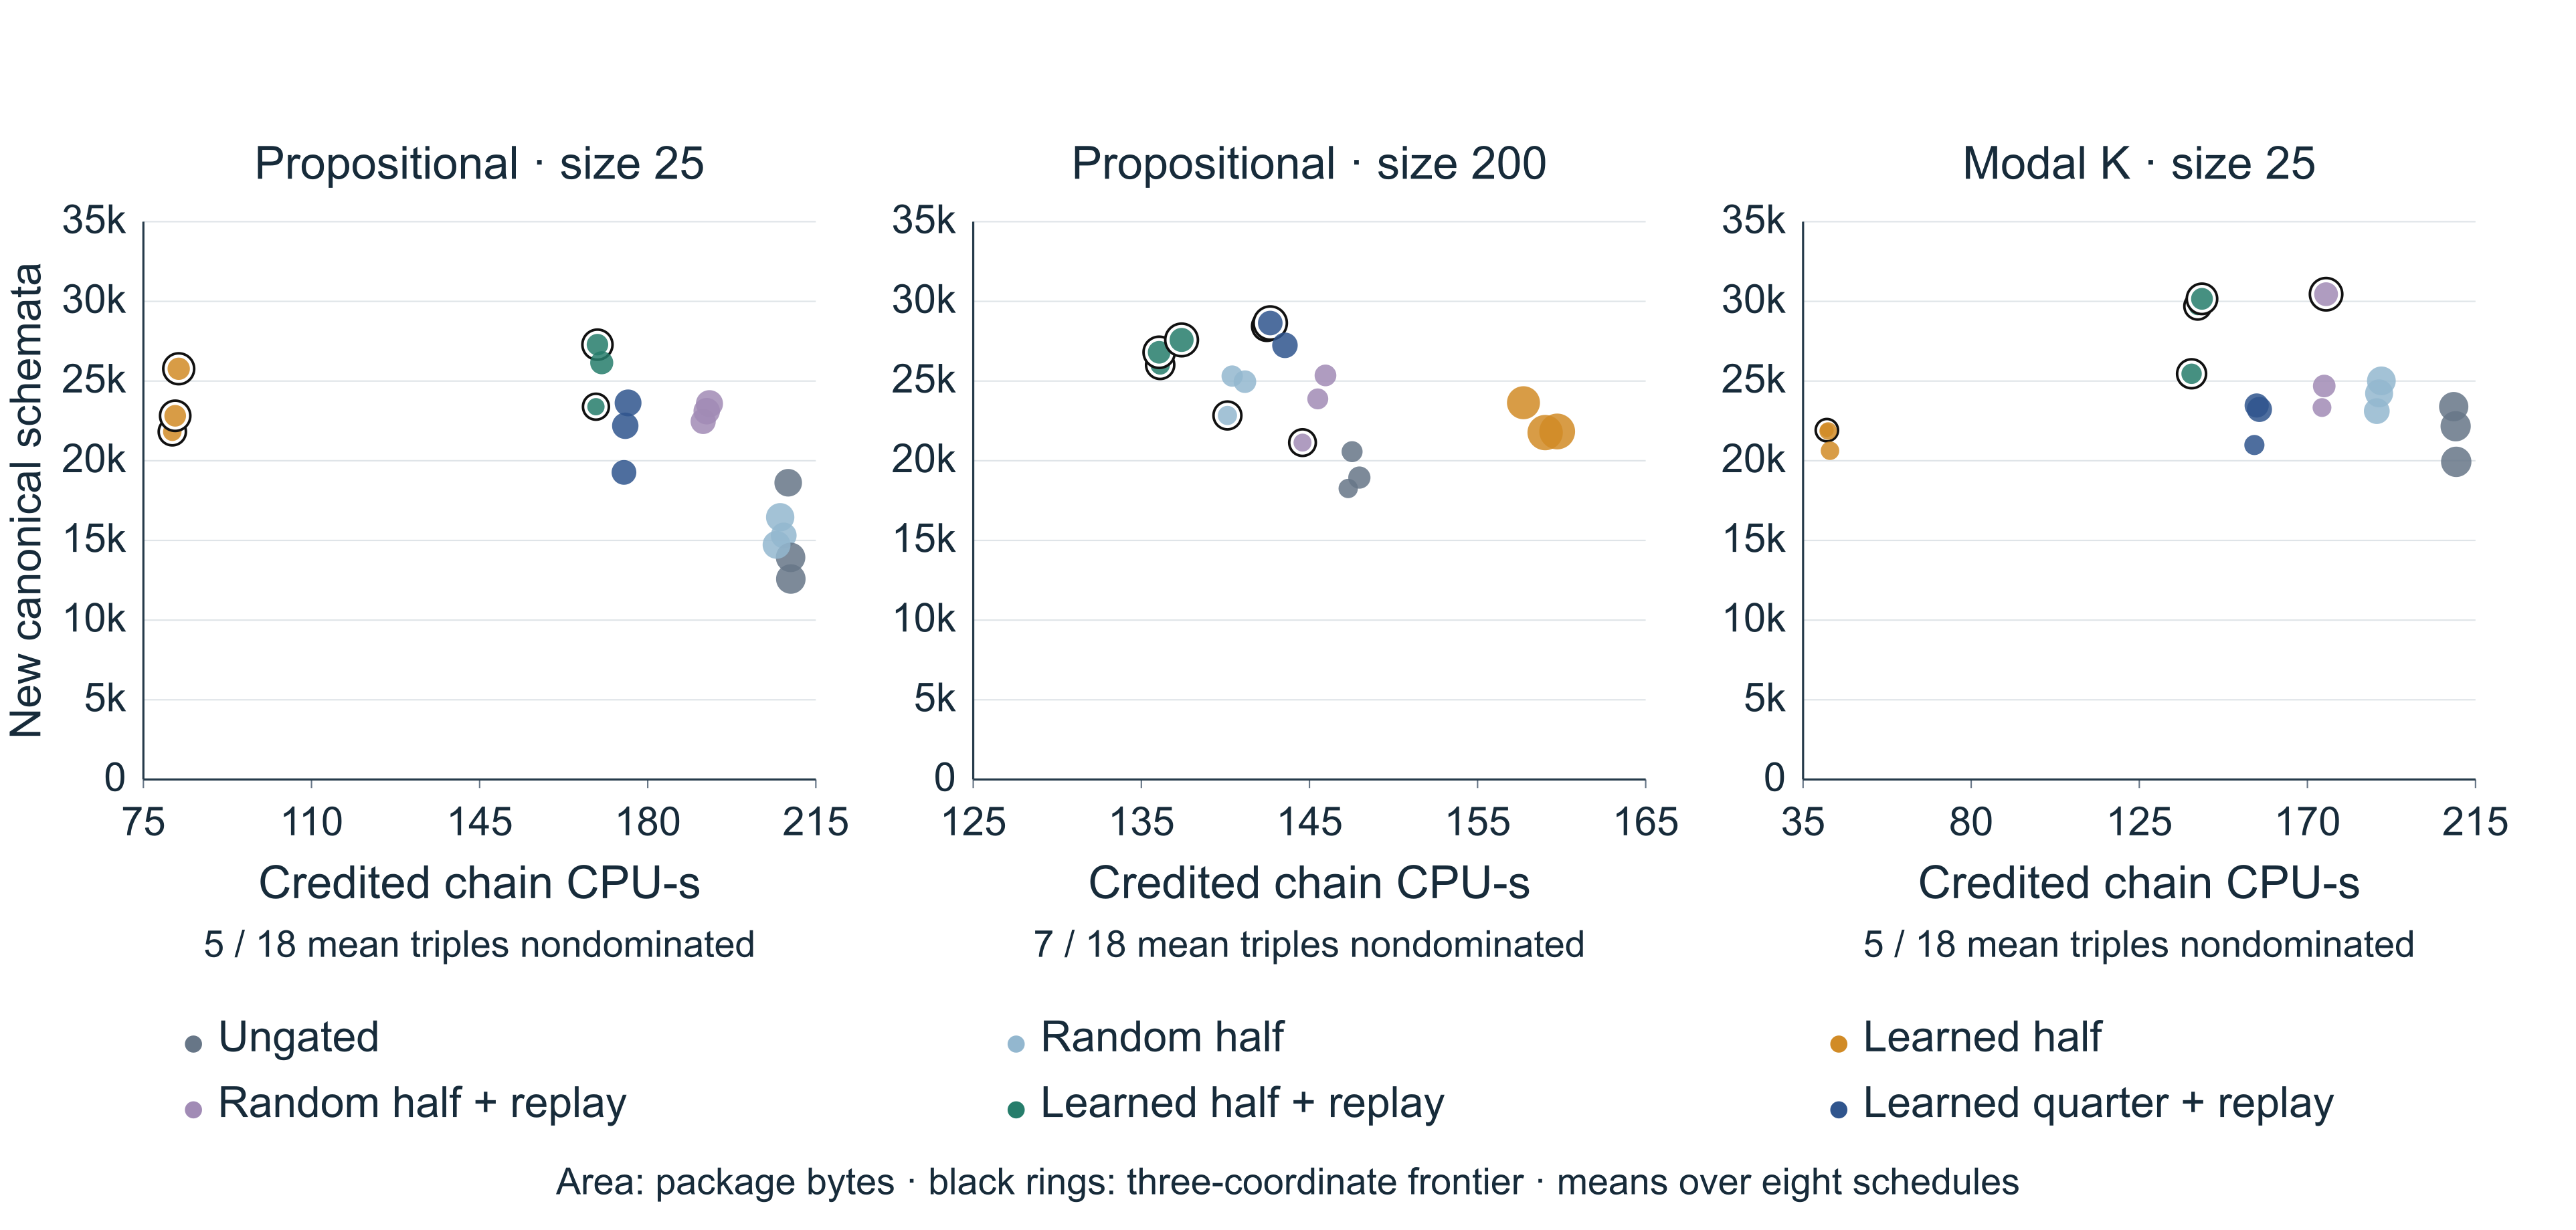
\includegraphics[width=\linewidth,height=.67\textheight,keepaspectratio]{Fig2.png}
\caption{Empirical Pareto trade-offs at a source ceiling of 180 CPU-seconds and continuation of 30 CPU-seconds. Colour identifies the pair policy, marker area indicates proof-backed package bytes, and outlines identify nondominated mean triples across CPU, bytes, and novelty. Each point averages eight scheduler states}\label{fig:2}
\end{figure}

These trade-offs favour different settings for different budgets. The learned half-filter without replay can cost less than replay at size 25, whereas replay yields more new schemata. More anchors or a later source slice need not improve continuation. The empirical frontier consequently supports a choice among useful finite skeletons, rather than a universal winner or an optimum beyond this grid.

\subsection*{7.2 Locked native comparison}\label{locked-native-comparison}
\addcontentsline{toc}{subsection}{7.2 Locked native comparison}

All 16 source blocks and 160 planned continuations finish both registered horizons and pass independent replay. Each table entry averages the two neutral continuers within a source, then averages the 16 sources. Initial coverage counts all 963 reference targets; both future columns count only the common initially uncovered residual within that source block. Derived-anchor counts exclude 29 basis roots and separate certificate-only support (Table 2).

\begingroup
\small
\setlength{\tabcolsep}{3pt}
\renewcommand{\arraystretch}{1.13}

\begin{longtable}[]{@{}
  >{\raggedright\arraybackslash}p{(\linewidth - 8\tabcolsep) * \real{0.2558}}
  >{\raggedleft\arraybackslash}p{(\linewidth - 8\tabcolsep) * \real{0.1701}}
  >{\raggedleft\arraybackslash}p{(\linewidth - 8\tabcolsep) * \real{0.1865}}
  >{\raggedleft\arraybackslash}p{(\linewidth - 8\tabcolsep) * \real{0.2259}}
  >{\raggedleft\arraybackslash}p{(\linewidth - 8\tabcolsep) * \real{0.1617}}@{}}
\caption{Initial coverage, further common-residual coverage, and anchors in the locked native comparison}\label{tab:5}\tabularnewline
\toprule\noalign{}
\begin{minipage}[b]{\linewidth}\raggedright
\textbf{Library}
\end{minipage} & \begin{minipage}[b]{\linewidth}\raggedleft
\textbf{Initial coverage}
\end{minipage} & \begin{minipage}[b]{\linewidth}\raggedleft
\textbf{New at 60 growth s}
\end{minipage} & \begin{minipage}[b]{\linewidth}\raggedleft
\textbf{New at 90 operational s}
\end{minipage} & \begin{minipage}[b]{\linewidth}\raggedleft
\textbf{Derived anchors}
\end{minipage} \\
\midrule\noalign{}
\endfirsthead
\toprule\noalign{}
\begin{minipage}[b]{\linewidth}\raggedright
\textbf{Library}
\end{minipage} & \begin{minipage}[b]{\linewidth}\raggedleft
\textbf{Initial coverage}
\end{minipage} & \begin{minipage}[b]{\linewidth}\raggedleft
\textbf{New at 60 growth s}
\end{minipage} & \begin{minipage}[b]{\linewidth}\raggedleft
\textbf{New at 90 operational s}
\end{minipage} & \begin{minipage}[b]{\linewidth}\raggedleft
\textbf{Derived anchors}
\end{minipage} \\
\midrule\noalign{}
\endhead
\bottomrule\noalign{}
\endlastfoot
Common core and short rules & 25.00 & 1.312 & 1.344 & 633.6 \\
Fixed extended repertoire & 29.00 & 1.594 & 1.625 & 675.0 \\
Random extended repertoire & 26.38 & 1.500 & 1.562 & 680.4 \\
Adaptive test variant & 27.88 & 1.656 & 1.688 & 673.4 \\
Whole fixed catalogue & 44.00 & 1.562 & 1.594 & 1282.3 \\
\end{longtable}

\endgroup

The whole fixed catalogue initially covers 44 targets, versus 29 for the fixed extended repertoire, but reaches 1.56 versus 1.59 new common-residual targets at 60 growth CPU-seconds. This contrast illustrates why initial coverage cannot rank future capability. The adaptive score chooses three distinct rule sets and reaches 1.656 new residual targets, yet its paired advantage over the quota-matched fixed repertoire averages only 0.0625 targets at either endpoint (Table 3).

\begingroup
\small
\setlength{\tabcolsep}{3pt}
\renewcommand{\arraystretch}{1.13}

\begin{longtable}[]{@{}
  >{\raggedright\arraybackslash}p{(\linewidth - 6\tabcolsep) * \real{0.3000}}
  >{\raggedleft\arraybackslash}p{(\linewidth - 6\tabcolsep) * \real{0.2400}}
  >{\raggedleft\arraybackslash}p{(\linewidth - 6\tabcolsep) * \real{0.2400}}
  >{\raggedleft\arraybackslash}p{(\linewidth - 6\tabcolsep) * \real{0.2200}}@{}}
\caption{Paired adaptive-minus-control differences and Holm-adjusted tests at both registered horizons}\label{tab:6}\tabularnewline
\toprule\noalign{}
\begin{minipage}[b]{\linewidth}\raggedright
\textbf{Adaptive minus control}
\end{minipage} & \begin{minipage}[b]{\linewidth}\raggedleft
\textbf{Difference at 60 growth s}
\end{minipage} & \begin{minipage}[b]{\linewidth}\raggedleft
\textbf{Difference at 90 operational s}
\end{minipage} & \begin{minipage}[b]{\linewidth}\raggedleft
\textbf{Holm adjusted p}
\end{minipage} \\
\midrule\noalign{}
\endfirsthead
\toprule\noalign{}
\begin{minipage}[b]{\linewidth}\raggedright
\textbf{Adaptive minus control}
\end{minipage} & \begin{minipage}[b]{\linewidth}\raggedleft
\textbf{Difference at 60 growth s}
\end{minipage} & \begin{minipage}[b]{\linewidth}\raggedleft
\textbf{Difference at 90 operational s}
\end{minipage} & \begin{minipage}[b]{\linewidth}\raggedleft
\textbf{Holm adjusted p}
\end{minipage} \\
\midrule\noalign{}
\endhead
\bottomrule\noalign{}
\endlastfoot
fixed & +0.06250 & +0.06250 & 1.000 \\
random & +0.15625 & +0.12500 & 1.000 \\
fixed all & +0.09375 & +0.09375 & 1.000 \\
\end{longtable}

\endgroup

Every Holm-adjusted p-value equals 1.000, and no contrast reaches the registered mean margin of one additional target at both clocks. We therefore retain fixed structural rules in the working architecture and do not attribute a confirmed gain to adaptive catalogue ranking. Appendix L reports the full paired comparison, statistical rule, and technical amendment.

The independent audit reconstructs 4,174,478 admission events and 2,846 hidden-support rediscovery witnesses, checks all target positions, and reproduces the endpoints and decision. These counts include repeated events across trajectories, not independent theorems. The comparison charges the full recorded catalogue to every arm under the shared backend; it does not test a specialised static implementation that avoids compiling unused entries.

\subsection*{7.3 Metamath and generated proof networks}\label{metamath-and-generated-proof-networks}
\addcontentsline{toc}{subsection}{7.3 Metamath and generated proof networks}

The network comparison follows the cumulative method through its delivered library and certificate support. Panel b uses the first source, 2026102201, with the quota-matched fixed structural repertoire. Appendix N presents the profiles of both variants and the separately preselected adaptive image. Both representatives follow the first-source convention, independently of target coverage, graph appearance, and power-law p-values.

All objects share the explicit native basis from the pinned \path{set.mm} revision \citep{MetamathSetMMPinned}: 25 logical or set-theoretic axioms and rules, six definitions, and 12 syntax assertions. Twenty-nine closed source schemata initialise search. The inherited proof-closed core contains 2,708 statements; the cumulative constructor continues that core, filters and revisits opportunities, applies reversible rot-pruning, compiles structural rules, and codes recurrent proofs. Panel b shows the delivered interface and every ancestor that its certificates require, not the full inherited archive. Appendix N records the new sources, projections, and metrics.

The first-source fixed library provides 675 derived anchors and 29 basis roots; 137 further vertices supply certificate-only support. Its projection therefore contains 841 vertices and 1,573 directed arcs. Across all 16 fixed sources, anchor counts range from 665 to 682, with a mean of 675.0; projected sizes range from 836 to 852. Hidden support does not confer search rights, and a verifier can expand every anchor to the original basis.

An arc runs from a premise to the conclusion that cites it. We omit primitive rule vertices and collapse repeated arcs in every object. Certificates retain joint premise roles, substitutions, and side conditions that this ordinary graph projection cannot express. The human fragment contains 2,306 named assertions whose actual proofs use only the declared basis, including assertions with essential hypotheses. Native vertices denote closed schemata with mandatory distinct-variable conditions. A shared basis does not eliminate the difference between named human steps and elementary native inferences.

The full reference enumerates all admitted MP steps through most-general unification and prescribed generalisations through proof height three, without skeleton-selection or formula-size cuts. Its 11,772 statements support both first-proof and all-inference projections. This reference supplies a complete finite slice of the stated operator, not all substitution instances, a deductive fixed point, or infinite closure of Zermelo--Fraenkel set theory with choice (ZFC). Panel b reaches certificate height 23; the comparison holds neither depth nor construction cost constant (Fig. 2).

\begin{figure}[!htbp]
\centering
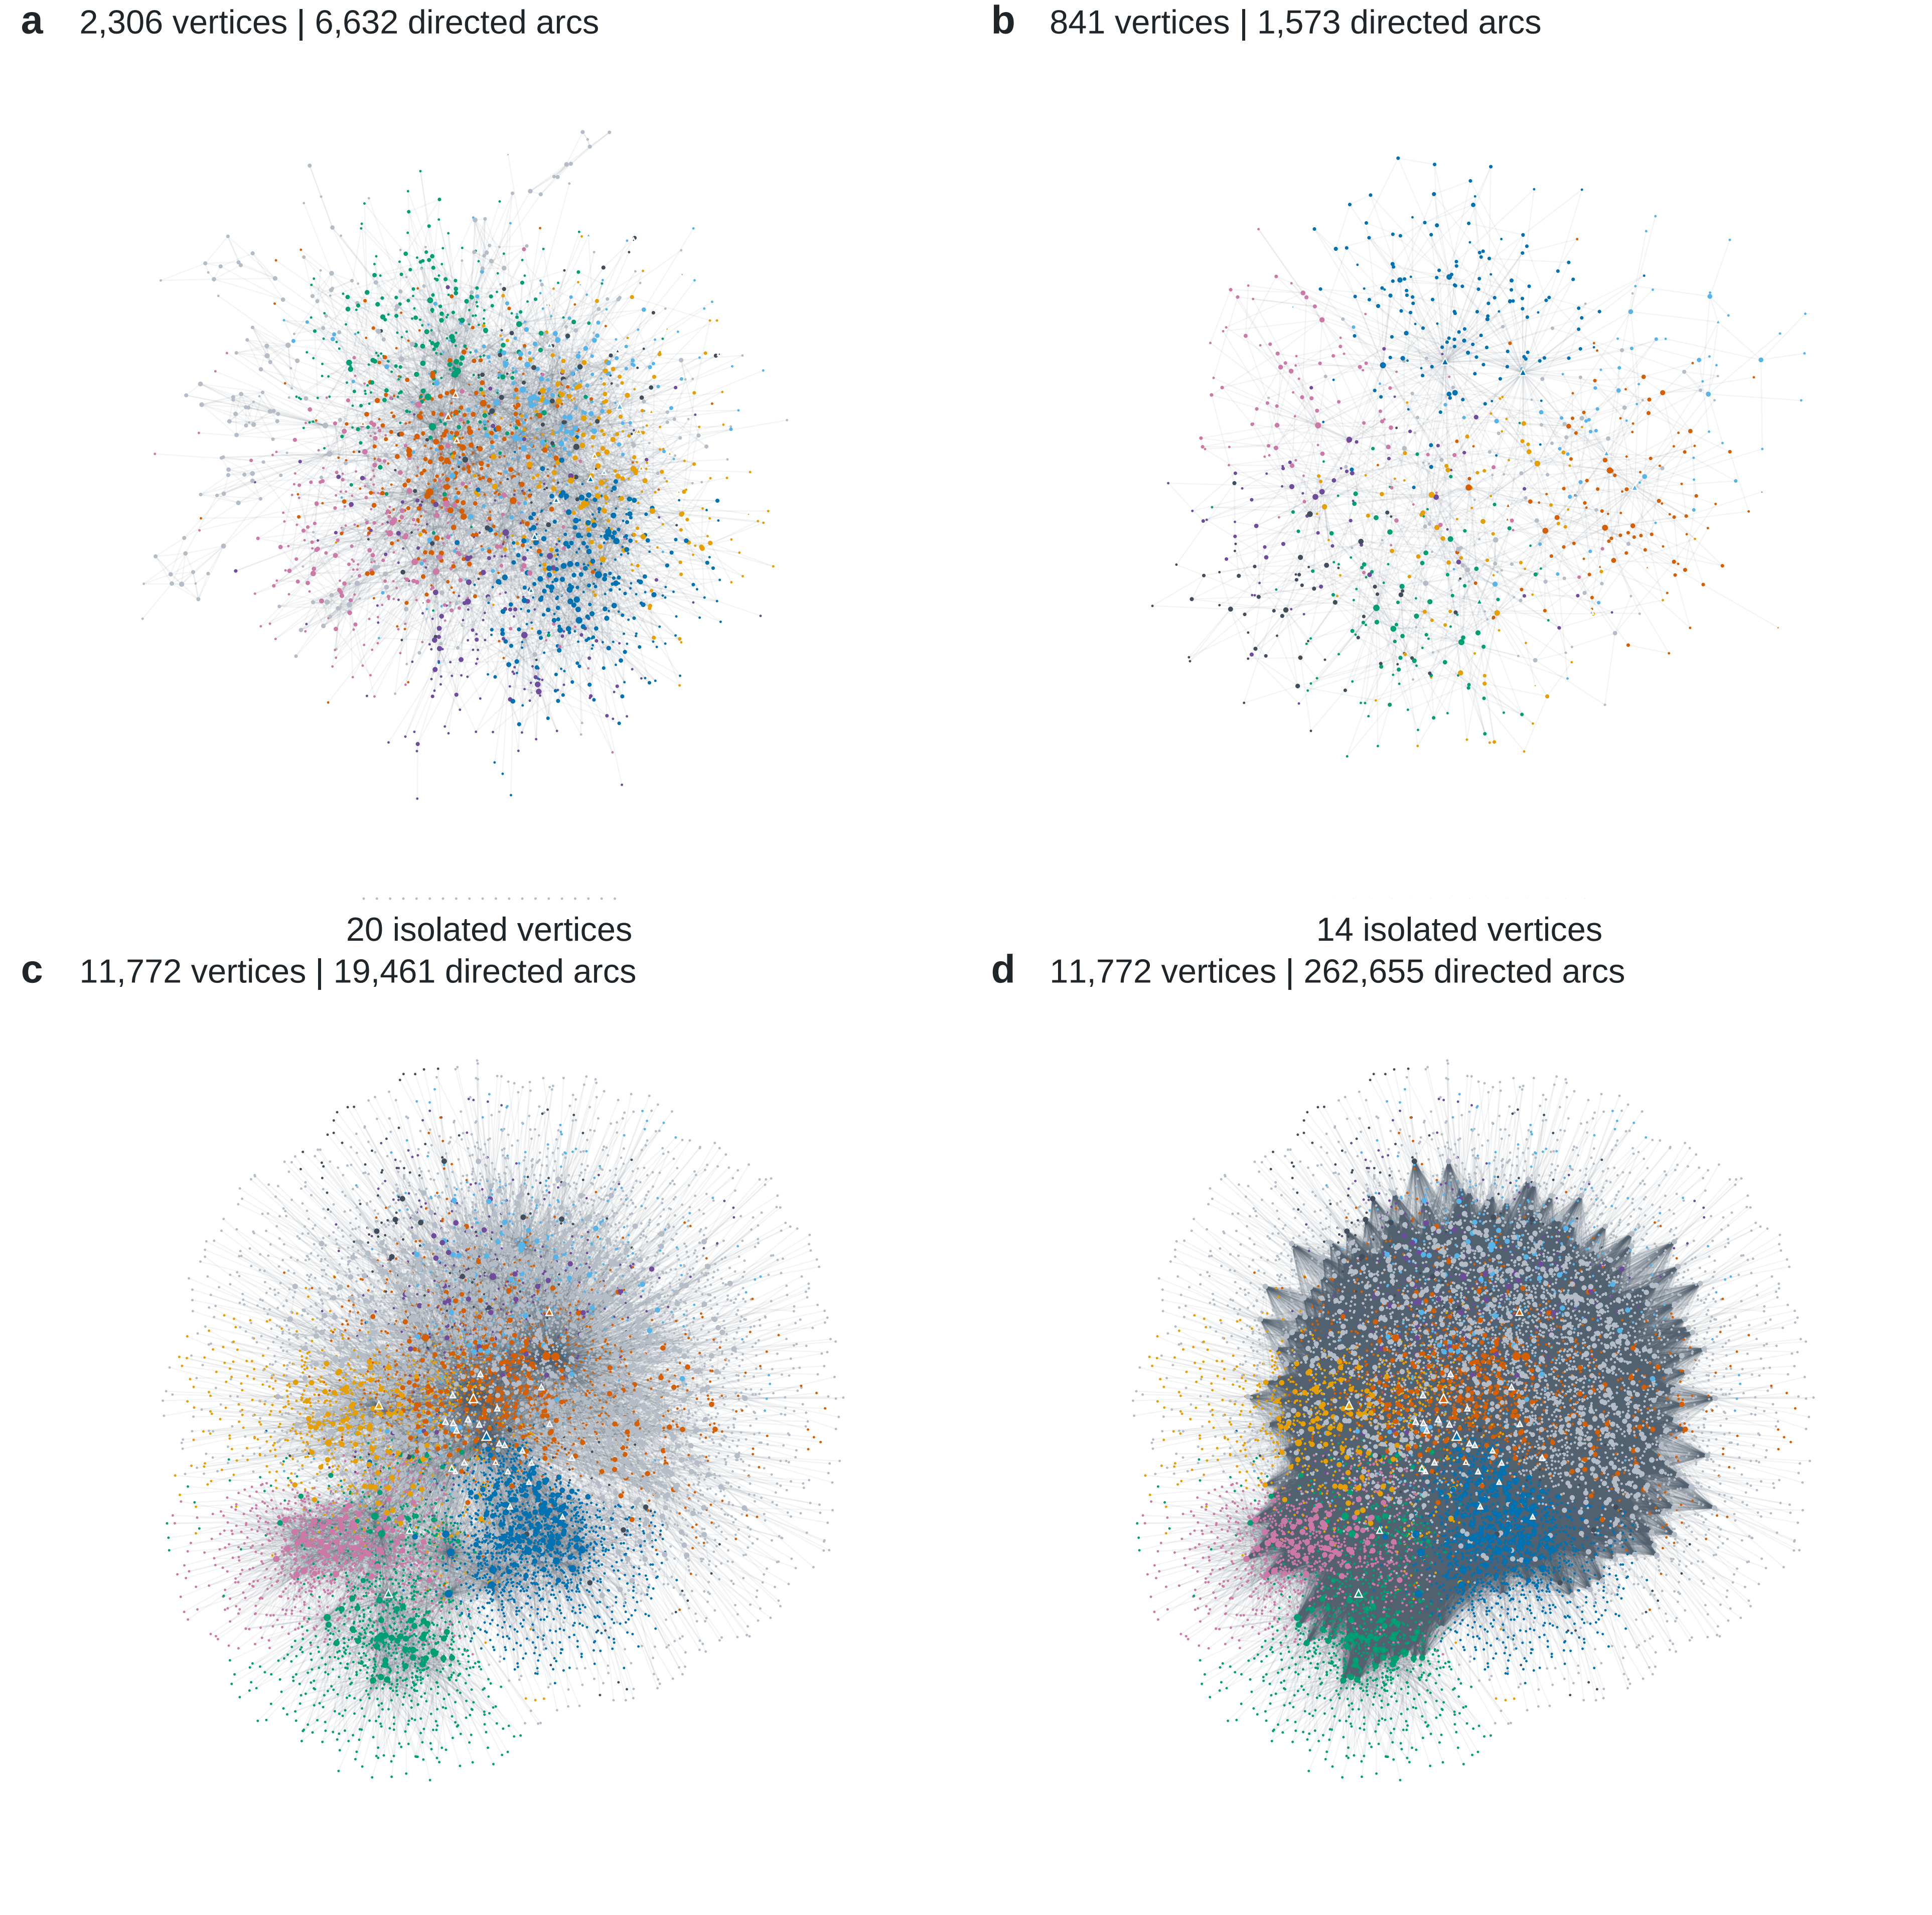
\includegraphics[width=\linewidth,height=.67\textheight,keepaspectratio]{Fig4.png}
\caption{Native proof networks on one explicit basis. a shows the compatible named Metamath fragment; b shows the first-source cumulative skeleton with fixed structural rules, including all certificate support; c shows first proofs in the complete height-three operator slice; d shows all enumerated inferences on those same vertices. Every vertex and unique undirected edge enters the drawing; only arrowheads disappear. Colours distinguish the eight largest communities in a, b, and c, with smaller communities in grey. d inherits c's coordinates, colours, and vertex areas; its tabulated modularity follows its own community search. Triangles mark the 29 basis roots. Areas increase with log reuse. Separate layouts do not measure comparable semantic distances}\label{fig:4}
\end{figure}

The representative skeleton reaches modularity 0.622, versus 0.539 across ten degree-preserving controls, and outgoing distinct-use degree yields a Gini coefficient of 0.731. Across the 16 fixed sources, modularity ranges from 0.622 to 0.629, with a mean of 0.625. These measurements characterise concentrated reuse and modular structure without promoting a single image to a mean result.

The new outgoing-degree profiles also differ from the earlier 2,708-vertex core. None of the 16 fixed-repertoire sources rejects the pure discrete power-law family at five percent; bootstrap p-values range from 0.24190 to 0.62575. The representative fits an exponent of 2.044719 from degree one, with 524 tail observations and p = 0.54640. Its other 317 vertices carry zero outgoing degree. On this same tail, the cutoff power law and rounded lognormal yield descriptive log likelihoods of \ensuremath{-}815.753 and \ensuremath{-}816.024, versus \ensuremath{-}818.182 for the pure power law. Compatibility with the pure family therefore does not select it uniquely or establish an infinite scale-free growth mechanism (Table 4).

\begingroup
\small
\setlength{\tabcolsep}{3pt}
\renewcommand{\arraystretch}{1.13}

\begin{longtable}[]{@{}
  >{\raggedright\arraybackslash}p{(\linewidth - 8\tabcolsep) * \real{0.3199}}
  >{\raggedleft\arraybackslash}p{(\linewidth - 8\tabcolsep) * \real{0.1700}}
  >{\raggedleft\arraybackslash}p{(\linewidth - 8\tabcolsep) * \real{0.1700}}
  >{\raggedleft\arraybackslash}p{(\linewidth - 8\tabcolsep) * \real{0.1700}}
  >{\raggedleft\arraybackslash}p{(\linewidth - 8\tabcolsep) * \real{0.1700}}@{}}
\caption{Network metrics for Metamath, the cumulative skeleton, and two complete height-three projections}\label{tab:7}\tabularnewline
\toprule\noalign{}
\begin{minipage}[b]{\linewidth}\raggedright
\textbf{Metric}
\end{minipage} & \begin{minipage}[b]{\linewidth}\raggedleft
\textbf{a Metamath}
\end{minipage} & \begin{minipage}[b]{\linewidth}\raggedleft
\textbf{b Cumulative skeleton}
\end{minipage} & \begin{minipage}[b]{\linewidth}\raggedleft
\textbf{c First proofs}
\end{minipage} & \begin{minipage}[b]{\linewidth}\raggedleft
\textbf{d All inferences}
\end{minipage} \\
\midrule\noalign{}
\endfirsthead
\toprule\noalign{}
\begin{minipage}[b]{\linewidth}\raggedright
\textbf{Metric}
\end{minipage} & \begin{minipage}[b]{\linewidth}\raggedleft
\textbf{a Metamath}
\end{minipage} & \begin{minipage}[b]{\linewidth}\raggedleft
\textbf{b Cumulative skeleton}
\end{minipage} & \begin{minipage}[b]{\linewidth}\raggedleft
\textbf{c First proofs}
\end{minipage} & \begin{minipage}[b]{\linewidth}\raggedleft
\textbf{d All inferences}
\end{minipage} \\
\midrule\noalign{}
\endhead
\bottomrule\noalign{}
\endlastfoot
Vertices \(N\) & 2306 & 841 & 11772 & 11772 \\
Directed arcs \(E\) & 6632 & 1573 & 19461 & 262655 \\
Largest-component vertices & 2286 & 827 & 11772 & 11772 \\
Isolated vertices & 20 & 14 & 0 & 0 \\
Mean local clustering \(C\) & 0.0689 & 0.0202 & 0.0347 & 0.3382 \\
Mean shortest path \(L\) & 4.137 & 4.177 & 4.334 & 3.213 \\
Diameter \(D\) & 11 & 8 & 6 & 4 \\
Modularity \(Q\) & 0.568 & 0.622 & 0.675 & 0.058 \\
Reference modularity \(Q_{0}\) & 0.401 & 0.539 & 0.599 & 0.053 \\
Small-world ratio \(\sigma_{DP}\) & 3.990 & 0.636 & 0.592 & 0.417 \\
Tail observations & 205 & 524 & 63 & 41 \\
Pure power law p & 0.09895 & 0.54640 & 0.01080 & 0.36490 \\
\end{longtable}

\endgroup

Table columns follow the figure panels. C, L, D, and Q refer to simple undirected projections. C assigns zero below degree two; L and D refer to the largest connected component and use every observed breadth-first-search (BFS) source. Panel a contains 20 isolates and panel b contains 14 unused basis roots; panels c and d remain connected. Q0 averages ten simple degree-preserving controls, with three Louvain starts for every observed and control graph. Panel b's control paths also use every source; the retained c and d controls estimate paths from 64 sources. The tail test for outgoing distinct-use degree fixes 20,000 bootstrap draws and refits both threshold and exponent. Appendix N reports all 32 new profiles and their scope.

The c--d pair isolates an edge-recording effect on identical statements: alternative edges raise clustering from 0.0347 to 0.3382, shorten the mean path from 4.334 to 3.213, and lower modularity from 0.675 to 0.058. No logical or vertex change explains that contrast. The ordinary proof-network profile therefore depends materially on how the representation records alternative derivations.

Newman \citep{Newman2003}, in \emph{The Structure and Function of Complex Networks}, treats degree heterogeneity, clustering, paths, and correlations as complementary features. Humphries and Gurney \citep{HumphriesGurney2008}, in \emph{Network `Small-World-Ness': A Quantitative Method for Determining Canonical Network Equivalence}, formalise the clustering--path comparison behind the small-world ratio. Under the declared degree-preserving reference, Metamath reaches a ratio of 3.990, whereas the skeleton reaches 0.636. Thus, the skeleton exhibits concentrated reuse, modular organisation, and a compatible conditional power-law tail, but its short paths do not establish small-world structure. These objects display distinct complex-network profiles rather than a division between networks and `mere graphs'. A conditional tail fit does not establish infinite scale invariance, and network metrics complement rather than replace future-use tests \citep{ClausetEtAl2009,BroidoClauset2019}. Ten null graphs support descriptive contrasts rather than a rank-test claim below five percent.

\section*{8 Discussion and scope}\label{discussion-and-scope}
\addcontentsline{toc}{section}{8 Discussion and scope}

The experiments establish that proof validity, compact proof code, and productive premise use answer different questions. The architecture preserves every accepted certificate while the policy changes which proven formulae can take part in new inferences. Internal controls measure the computational consequences of that change. Fragment reuse alone does not determine the return from an active slot, as the utility problem for acquired knowledge predicts \citep{Minton1990Utility}.

The coding library stores exact closed first proofs rather than shortest proofs. The structural extension separately derives general closed schemata by discharging open MP boundaries. The archive already shares identical subproofs in a directed acyclic graph (DAG), so shorter expanded terms do not demonstrate further compression of that graph. Repeated fragment use and conservative lemma synthesis preserve formal meaning; the costed future-growth test measures their operational value.

Human references expose differences that raw formula counts conceal.  The locked comparison evaluates a previously unscored 963-target POI subset only after every search trajectory freezes; a separate independent audit then checks the outcome. None of these corpora supplies a complete modal reference or an assessment of the whole mathematical value of the generated library.

The native network study adds a structural result to the operational evidence. A proof-closed skeleton exhibits modular organisation and concentrated reuse, whereas the fixed-vertex reference shows that alternative proof edges can strongly alter the same network metrics. Verified certificates, human-statement coverage, and measured continuation complement this structural profile. The native network study and the earlier pair-selection trajectories retain their separate scopes.

The combinatorial claims also require distinct scopes. The exponential lower bound counts explicit theorem instances, whereas the result for canonical schemata establishes only unboundedness. Neither the theorems nor finite runs establish non-computability of a bounded slice, exponential growth of schemata, or the limiting topology of an infinite proof space. Since the two logics change their language, axioms, and rules together, they do not isolate logic alone as a cause.

The native comparison supplies a reproducible operating configuration with fixed structural rules. Goal-directed proof search and control towards prescribed graph properties define the next two research tracks. For knowledge-based AI, our method preserves certified knowledge, changes which statements inference may use, and accounts for the required resources.

\section*{9 Conclusions}\label{conclusions}
\addcontentsline{toc}{section}{9 Conclusions}

We formulate the direct, inverse, and control cognition problems for formal knowledge. The direct cognition problem generates a proof skeleton without a final target theorem. 

We develop a cumulative method that generates a semantic skeleton through checkable anchor statements and expandable proofs. The method addresses the direct cognition problem by separating archived proofs, active premises, and reusable lemma entries. Premise filtering, deferred replay, and reversible deactivation regulate immediate work; positive-marginal coding retains recurrent proof fragments; a structural compiler derives general lemma schemata with elementary certificates. The theoretical results establish conservative proof recovery and the output obstruction to complete explicit storage under fixed capacity.

The experiments assess future capability rather than count retained formulae alone. In the 144-source continuation panel, learned pair selection with deferred replay raises mean novelty over ungated growth by 95.8\% and 30.3\% in the two propositional regimes, with eight positive pairs in each and lower mean credited chain CPU. Modal outcomes and resource guards delimit the claim. Empirical Pareto sets retain the finite trade-offs among CPU, package bytes, and future output rather than name a universal winner.

The native architecture carries the accumulated method onto an explicit Metamath basis with checked structural rules and controlled access to certificate support. The locked 963-target test completes 160 continuations across 16 source blocks and passes independent replay. The registered comparison does not confirm an adaptive advantage; fixed structural rules supply the final repertoire. The locked comparison separates initial coverage from newly reached reference statements.

The new network comparison characterises the resulting certified skeleton alongside human mathematics and finite exhaustive growth. The first-source fixed skeleton contains 841 certificate vertices and reaches modularity 0.622; all 16 profiles quantify variation. Their outgoing-degree diagnostics do not reject a pure power-law tail, although alternative models also fit and the finite experiment establishes no limiting law. On the identical 11,772 vertices of the complete height-three slice, alternative proof edges raise clustering from 0.0347 to 0.3382 while lowering modularity from 0.675 to 0.058. These measurements connect useful finite proof libraries to network structure.

The principal result answers the direct question through an executable proof-preserving method, a future-use criterion, and an explicit cost account. It supports continued inference from finite certified skeletons in the tested regimes and connects their operational use to measurable network structure. 

\section*{10 Reproducibility}\label{reproducibility}
\addcontentsline{toc}{section}{10 Reproducibility}

The reproducibility records link every new numerical claim to its protocol, code, and source results. All 16 blind receipts, the one-shot evaluation, the completed pipeline, and the independent review refer to the corrected seal in Appendix L. The auditor rechecks permitted inference, target-instance certificates, common residuals, and the statistical decision. 

\section*{Statements and Declarations}

\subsection*{Data availability}\label{data-availability}
\addcontentsline{toc}{subsection}{Data availability}

We publicly provide source code for the main native workflow, self-contained tests, and compact checked results at https://github.com/nnevdokimov/certified-proof-skeleton. Frozen packages and the editorial manifest identify the protocols, code versions, input hashes, and numerical sources. We do not yet provide the complete experimental record in a permanent archive. The source release does not include a reuse licence; third-party inputs retain their original licence requirements.

\subsection*{Conflicts of interest}\label{conflicts-of-interest}
\addcontentsline{toc}{subsection}{Conflicts of interest}

The authors declare no conflict of interest concerning this article.

\subsection*{Funding}\label{funding}
\addcontentsline{toc}{subsection}{Funding}

The research leading to these results received funding from the Basic Research Program at HSE University {[}HSE-BR-2025-025{]}.

\subsection*{Acknowledgments}\label{acknowledgments}
\addcontentsline{toc}{subsection}{Acknowledgments}

We used the HSE University supercomputer to conduct the computational research.

\begin{thebibliography}{37}
\bibitem{MetamathSetMMPinned} Metamath Project. (2026). \emph{set.mm: ZFC set theory database, fixed experimental version}. \url{https://github.com/metamath/set.mm/commit/584b6852f57f281e9be1793332f1e52e077693c8}

\bibitem{BachmairGanzinger2001} Bachmair, L., \& Ganzinger, H. (2001). Resolution theorem proving. In J. A. Robinson \& A. Voronkov (Eds.), \emph{Handbook of automated reasoning} (pp. 19--99). Elsevier. \url{https://doi.org/10.1016/B978-044450813-3/50004-7}

\bibitem{Wernhard2026} Wernhard, C. (2026). Generating theorems by generating proof structures. \emph{Automated Reasoning: IJCAR 2026, Lecture Notes in Computer Science}, \emph{16688}, 41--61. \url{https://doi.org/10.1007/978-3-032-32589-1_3}

\bibitem{Schulz2002} Schulz, S. (2002). E -- a brainiac theorem prover. \emph{AI Communications}, \emph{15}(2--3), 111--126. \url{https://doi.org/10.3233/EAI-2002-260}

\bibitem{KovacsVoronkov2013} Kov\'{a}cs, L., \& Voronkov, A. (2013). First-order theorem proving and Vampire. \emph{Computer Aided Verification}, 1--35. \url{https://doi.org/10.1007/978-3-642-39799-8_1}

\bibitem{RiazanovVoronkov2003LRS} Riazanov, A., \& Voronkov, A. (2003). Limited resource strategy in resolution theorem proving. \emph{Journal of Symbolic Computation}, \emph{36}(1--2), 101--115. \url{https://doi.org/10.1016/S0747-7171(03)00040-3}

\bibitem{HoderVoronkov2011} Hoder, K., \& Voronkov, A. (2011). Sine qua non for large theory reasoning. \emph{Automated Deduction -- CADE-23}, 299--314. \url{https://doi.org/10.1007/978-3-642-22438-6_23}

\bibitem{BlanchetteEtAl2016} Blanchette, J. C., Greenaway, D., Kaliszyk, C., K\"{u}hlwein, D., \& Urban, J. (2016). A learning-based fact selector for Isabelle/HOL. \emph{Journal of Automated Reasoning}, \emph{57}(3), 219--244. \url{https://doi.org/10.1007/s10817-016-9362-8}

\bibitem{JakubuvUrban2017} Jakub\r{u}v, J., \& Urban, J. (2017). ENIGMA: Efficient learning-based inference guiding machine. \emph{Intelligent Computer Mathematics}, 292--302. \url{https://doi.org/10.1007/978-3-319-62075-6_20}

\bibitem{Colton2002} Colton, S. (2002). \emph{Automated theory formation in pure mathematics}. Springer. \url{https://doi.org/10.1007/978-1-4471-0147-5}

\bibitem{SmallboneEtAl2017} Smallbone, N., Johansson, M., Claessen, K., \& Algehed, M. (2017). Quick specifications for the busy programmer. \emph{Journal of Functional Programming}, \emph{27}, e18. \url{https://doi.org/10.1017/S0956796817000090}

\bibitem{ClaessenEtAl2013} Claessen, K., Johansson, M., Ros\'{e}n, D., \& Smallbone, N. (2013). Automating inductive proofs using theory exploration. \emph{Automated Deduction -- CADE-24, Lecture Notes in Computer Science}, \emph{7898}, 392--406. \url{https://doi.org/10.1007/978-3-642-38574-2_27}

\bibitem{JohanssonEtAl2014} Johansson, M., Ros\'{e}n, D., Smallbone, N., \& Claessen, K. (2014). Hipster: Integrating theory exploration in a proof assistant. \emph{Intelligent Computer Mathematics}, 108--122. \url{https://doi.org/10.1007/978-3-319-08434-3_9}

\bibitem{SingherItzhaky2021} Singher, E., \& Itzhaky, S. (2021). Theory exploration powered by deductive synthesis. \emph{Computer Aided Verification, Lecture Notes in Computer Science}, \emph{12760}, 125--148. \url{https://doi.org/10.1007/978-3-030-81688-9_6}

\bibitem{McCaslandBundySmith2017} McCasland, R. L., Bundy, A., \& Smith, P. F. (2017). MATHsAiD: Automated mathematical theory exploration. \emph{Applied Intelligence, 47}, 585--606. \url{https://doi.org/10.1007/s10489-017-0954-8}

\bibitem{WernhardBibel2024} Wernhard, C., \& Bibel, W. (2024). Investigations into proof structures. \emph{Journal of Automated Reasoning}, \emph{68}, 24. \url{https://doi.org/10.1007/s10817-024-09711-8}

\bibitem{RawsonEtAl2023} Rawson, M., Wernhard, C., Zombori, Z., \& Bibel, W. (2023). Lemmas: Generation, selection, application. \emph{Automated Reasoning with Analytic Tableaux and Related Methods}, 153--174. \url{https://doi.org/10.1007/978-3-031-43513-3_9}

\bibitem{WernhardZombori2025} Wernhard, C., \& Zombori, Z. (2025). Mathematical knowledge bases as grammar-compressed proof terms: Exploring Metamath proof structures. \emph{arXiv Preprint arXiv:2505.12305}. \url{https://doi.org/10.48550/arXiv.2505.12305}

\bibitem{Minton1990Utility} Minton, S. (1990). Quantitative results concerning the utility of explanation-based learning. \emph{Artificial Intelligence}, \emph{42}(2--3), 363--391. \url{https://doi.org/10.1016/0004-3702(90)90059-9}

\bibitem{KaliszykUrban2015} Kaliszyk, C., \& Urban, J. (2015). Learning-assisted theorem proving with millions of lemmas. \emph{Journal of Symbolic Computation}, \emph{69}, 109--128. \url{https://doi.org/10.1016/j.jsc.2014.09.032}

\bibitem{WangEtAl2023Lego} Wang, H., Xin, H., Zheng, C., Liu, Z., Cao, Q., Huang, Y., Xiong, J., Shi, H., Xie, E., Yin, J., Li, Z., \& Liang, X. (2024). LEGO-Prover: Neural theorem proving with growing libraries. \emph{The Twelfth International Conference on Learning Representations}. \url{https://proceedings.iclr.cc/paper_files/paper/2024/hash/85dca46374dc0f27b4bb5f265b3d17f0-Abstract-Conference.html}

\bibitem{YangEtAl2023} Yang, K., Swope, A., Gu, A., Chalamala, R., Song, P., Yu, S., Godil, S., Prenger, R., \& Anandkumar, A. (2023). LeanDojo: Theorem proving with retrieval-augmented language models. \emph{Advances in Neural Information Processing Systems: Datasets and Benchmarks}. \url{https://doi.org/10.52202/075280-0944}

\bibitem{PoesiaEtAl2024} Poesia, G., Broman, D., Haber, N., \& Goodman, N. D. (2024). Learning formal mathematics from intrinsic motivation. \emph{Advances in Neural Information Processing Systems}, \emph{37}. \url{https://doi.org/10.52202/079017-1362}

\bibitem{OtaEtAl2026} Ota, K., Osa, T., \& Harada, T. (2026). Self-supervised theorem discovery in a formal axiomatic system. \emph{arXiv Preprint arXiv:2606.28747}. \url{https://doi.org/10.48550/arXiv.2606.28747}

\bibitem{LinEtAl2024} Lin, X., Cao, Q., Huang, Y., Yang, Z., Liu, Z., Li, Z., \& Liang, X. (2024). ATG: Benchmarking automated theorem generation for generative language models. \emph{Findings of the Association for Computational Linguistics: NAACL 2024}, 4465--4480. \url{https://doi.org/10.18653/v1/2024.findings-naacl.279}

\bibitem{TomaszukEtAl2023} Tomaszuk, D., Szeremeta, \L{}., \& Korni\l{}owicz, A. (2023). MMLKG: Knowledge graph for mathematical definitions, statements and proofs. \emph{Scientific Data}, \emph{10}, 791. \url{https://doi.org/10.1038/s41597-023-02681-3}

\bibitem{LiEtAl2026} Li, X., Peng, N., Severini, S., \& Shafto, P. (2026). The network structure of mathlib. \emph{arXiv Preprint arXiv:2604.24797}. \url{https://doi.org/10.48550/arXiv.2604.24797}

\bibitem{FlajoletSedgewick2009} Flajolet, P., \& Sedgewick, R. (2009). \emph{Analytic combinatorics}. Cambridge University Press. \url{https://doi.org/10.1017/CBO9780511801655}

\bibitem{CookReckhow1979} Cook, S. A., \& Reckhow, R. A. (1979). The relative efficiency of propositional proof systems. \emph{Journal of Symbolic Logic}, \emph{44}(1), 36--50. \url{https://doi.org/10.2307/2273702}

\bibitem{Newman2003} Newman, M. E. J. (2003). The structure and function of complex networks. \emph{SIAM Review}, \emph{45}(2), 167--256. \url{https://doi.org/10.1137/S003614450342480}

\bibitem{HumphriesGurney2008} Humphries, M. D., \& Gurney, K. (2008). Network `small-world-ness': A quantitative method for determining canonical network equivalence. \emph{PLoS ONE}, \emph{3}(4), e0002051. \url{https://doi.org/10.1371/journal.pone.0002051}

\bibitem{ClausetEtAl2009} Clauset, A., Shalizi, C. R., \& Newman, M. E. J. (2009). Power-law distributions in empirical data. \emph{SIAM Review}, \emph{51}(4), 661--703. \url{https://doi.org/10.1137/070710111}

\bibitem{BroidoClauset2019} Broido, A. D., \& Clauset, A. (2019). Scale-free networks are rare. \emph{Nature Communications}, \emph{10}, 1017. \url{https://doi.org/10.1038/s41467-019-08746-5}

\end{thebibliography}
\end{document}
